% -*- latex -*-

\chapter{Basic Usage}
\label{chap:Basic_Usage}

In this chapter we describe in greater detail the basic features of \IceT.
The tutorial given in Chapter~\ref{chap:Tutorial} is a good place to
start building your applications.  You can then consult this chapter and
later ones for more details on the operations as well as descriptions of
further features.

Prototypes for the majority of \IceT types, functions, and identifiers can
be found in the \index{ice-t.h}\index{GL/ice-t.h}\textC{GL/ice-t.h} header
file.  You will also almost always need to include the header
\index{ice-t\_mpi.h}\index{GL/ice-t\_mpi.h}\textC{GL/ice-t\_mpi.h}.
Chapter~\ref{chap:Communicators} provides more details on this latter
header file's function.
\begin{code}
#include <GL/ice-t.h>
#include <GL/ice-t_mpi.h>
\end{code}

\section{The State Machine}
\label{sec:Basic_Usage:The_State_Machine}

\index{state|(}

The \IceT API borrows many concepts from \index{OpenGL}OpenGL.  One major
concept taken is that of a state machine.  At all times \IceT maintains a
current state.  The state can influence the operations that \IceT makes,
and \IceT's operations can modify the state.

\index{context!\IceT|(}
\IceT can manage multiple collections of state at the same time.  It does
this by associating each state with a
\keyterm{context}.  At any given time, there is at
most one active context.  Any \IceT function called works using the current
active context.

Contexts are created and destroyed with \CFunc{icetCreateContext} and
\CFunc{icetDestroyContext}, respectively.

\begin{Table}{3}
  \CType{IceTContext}\textC{ }\CFunc{icetCreateContext}\textC{(}&\CType{IceTCommunicator}&\CArg{comm}\quad\textC{);}
\end{Table}
\begin{Table}{3}
  \textC{void }\CFunc{icetDestroyContext}\textC{(}&\CType{IceTContext}&\CArg{context}\quad\textC{;}
\end{Table}

These functions work with an object of type \CType{IceTContext}.
\CType{IceTContext} is an opaque type; you are not meant to directly access
it.  Instead, you pass the object to functions to do the work for you.

The \CFunc{icetCreateContext} function requires an object of type
\CType{IceTCommunicator}.  This is another opaque type that is described in
more detail in Chapter~\ref{chap:Communicators}.  For now, just know that
you can create one from an MPI communicator using the
\CFunc{icetCreateMPICommunicator} function.

\begin{Table}{3}
  \CType{IceTCommunicator}\textC{ }\CFunc{icetCreateMPICommunicator}\textC{(} \\
  \qquad\qquad\qquad\qquad\qquad\qquad\qquad\qquad\qquad\qquad\qquad
  \CTypeExternal{MPI\_Comm}\quad\CArg{mpi\_comm}\quad\textC{);}
\end{Table}
\begin{Table}{3}
  \textC{void }\CFunc{icetDestroyMPICommunicator}\textC{(}&\CType{IceTCommunicator}&\CArg{comm}\quad\textC{);}
\end{Table}

The following code gives the common boilerplate for setting up your initial
\IceT context.

\begin{code}
#include <GL/ice-t.h>
#include <GL/ice-t_mpi.h>

int main(int argc, char **argv)
{
  IceTCommunicator icetComm;
  IceTContext icetContext;

  /* Setup MPI. */
  MPI_Init(&argc, &argv);

  /* Setup an IceT context.  If we are only creating one, this context will
   * always be current. */
  icetComm = icetCreateMPICommunicator(MPI_COMM_WORLD);
  icetContext = icetCreateContext(icetComm);
  icetDestroyMPICommunicator(icetComm);

  /* Start your parallel rendering program here. */

  /* Cleanup IceT and MPI. */
  icetDestroyContext(icetContext);
  MPI_Finalize();

  return 0;
}
\end{code}

Any number of contexts may be created, each with its own associated state.
At any given time, a single given context is
\index{content!current}\keyterm{current}.  All \IceT operations are applied
with the state attached to the current context.  A handle to the current
\IceT context can be retrieved with the \CFunc{icetGetContext} function,
and he current context can be changed by using the \CFunc{icetSetContext}
function.

\begin{Table}{3}
  \CType{IceTContext}\textC{ }\CFunc{icetGetContext}\textC{(}&\textC{void}&\textC{);}
\end{Table}

\begin{Table}{3}
  \textC{void }\CFunc{icetSetContext}\textC{(}&\CType{IceTContext}&\CArg{context}\quad\textC{);}
\end{Table}

Changing the context is a fast and easy way to swap states.  This could be
used, for example, to switch between rendering modes.  One context could be
used for a full resolution image, and another could use
\index{image~inflation}\keyterm{image inflation} (described in
Chapter~\ref{sec:Customizing_Compositing:Image_Inflation}) to make faster
but coarser images during interaction.

When a context is created, its state is initialized to default values.  You
can effectively ``duplicate'' a context by copying the state of one context
to another using the \CFunc{icetCopyState} function.

\begin{Table}{3}
  \textC{void }\CFunc{icetCopyState}\textC{(}&\CType{IceTContext}&\CArg{dest}\textC{,} \\
      &\CType{IceTContext}&\CArg{src}\quad\textC{);}
\end{Table}

\index{context!\IceT|)}

The state of a context comprises a group of key/value pairs.  The state can
be queried by using any of the \CFunc{icetGet} functions.

\begin{Table}{3}
  \textC{void }\icetGetDoublev\textC{(}&\textC{GLenum}&\CArg{pname}\textC{,} \\
    &\textC{GLdouble *}&\CArg{params}\quad\textC{);}
\end{Table}

\begin{Table}{3}
  \textC{void }\icetGetFloatv\textC{(}&\textC{GLenum}&\CArg{pname}\textC{,} \\
      &\textC{GLfloat *}&\CArg{params}\quad\textC{);}
\end{Table}

\begin{Table}{3}
  \textC{void }\icetGetIntegerv\textC{(}&\textC{GLenum}&\CArg{pname}\textC{,} \\
      &\textC{GLint *}&\CArg{params}\quad\textC{);}
\end{Table}

\begin{Table}{3}
  \textC{void }\icetGetBooleanv\textC{(}&\textC{GLenum}&\CArg{pname}\textC{,} \\
      &\textC{GLboolean *}&\CArg{params}\quad\textC{);}
\end{Table}

\begin{Table}{3}
  \textC{void }\icetGetPointerv\textC{(}&\textC{GLenum}&\CArg{pname}\textC{,} \\
      &\textC{GLvoid **}&\CArg{params}\quad\textC{);}
\end{Table}

The valid keys that can be used in the \CFunc{icetGet} functions are listed
in the \CFunc{icetGet} documentation starting on
page~\pageref{manpage:icetGet}.  There is no way to directly set these
state variables.  Instead, they are set either by \IceT configuration
functions or indirectly as part of the operation of \IceT.  The
documentation for \CFunc{icetGet} also describes which functions can be
used to set each state entry (assuming the user has control of that state
entry).

There is a special set of state entries that toggle \IceT options.  Although
you can query this state with the \icetGetBooleanv function, it is more
typical to use the \CFunc{icetIsEnabled} function.  Also unlike the other
state variables, these variables can be directly manipulated with the
\CFunc{icetEnable} and \CFunc{icetDisable} functions.

\begin{Table}{4}
  \textC{GLboolean }\CFunc{icetIsEnabled}\textC{(}&\textC{GLenum}&\CArg{pname}&\textC{);}
\end{Table}

\begin{Table}{4}
  \textC{void }\icetEnable&\textC{(}&\textC{GLenum}&\CArg{pname}\quad\textC{);}
\end{Table}

\begin{Table}{4}
  \textC{void }\icetDisable&\textC{(}&\textC{GLenum}&\CArg{pname}\quad\textC{);}
\end{Table}

The options queried with \CFunc{icetIsEnabled} and manipulated with
\CFunc{icetEnable} and \CFunc{icetDisable} are listed in the
\CFunc{icetEnable} documentation starting on
page~\pageref{manpage:icetEnable}.

\index{state|)}


\section{Diagnostics}
\label{sec:Basic_Usage:Diagnostics}

\index{diagnostics|(}

The \IceT library has a mechanism for reporting diagnostics.  There are
three levels of diagnostics.  \index{error}\keyterm{Errors} are anomalous
conditions that \IceT considers a critical failure.  An occurrence of an
error generally means that the future \IceT operations will have undefined
behavior.  When \IceT is compiled in debug mode, a seg fault is
intentionally raised when an error occurs to make it easier to attach a
debugger to the point where the error occurred.

\index{warning}\keyterm{Warnings} are detections of anomalous conditions
that are not as severe as errors.  When a warning occurs, the current
operation may produce the incorrect results, but future operations should
continue to work.

\IceT also can also provide a large volume of \index{debug}\keyterm{debug}
messages.  These messages simply indicate the status of \IceT operations as
they progress.  They are generally of no use to anyone who is not trying to
develop or debug \IceT operations.

\IceT diagnostics are controlled with the \CFunc{icetDiagnostics} function.

\begin{Table}{3}
  \textC{void }\CFunc{icetDiagnostics}\textC{(}&\textC{GLbitfield}&\CArg{mask}\quad\textC{);}
\end{Table}

The \CFunc{icetDiagnostics} function takes a set of flags that can me or-ed
together.  The diagnostics for errors, warnings, and debug statements can
be set by passing the \CEnum{ICET\_DIAG\_ERRORS},
\CEnum{ICET\_DIAG\_WARNINGS}, and \CEnum{ICET\_DIAG\_DEBUG} flags, respectively.
Turning on warnings implicitly turns on errors and turning on debug
statements implicitly turns on errors and warnings (although there is no
problem with redundantly specifying these flags).

\IceT has the ability to report diagnostics either on all processes or only
on the \index{root~process}\keyterm{root process} (the process with rank
0).  This behavior is controlled by the \CEnum{ICET\_DIAG\_ROOT\_NODE} and
\CEnum{ICET\_DIAG\_ALL\_NODES} flags.  Many diagnostic messages occur on
all nodes when they occur, so reporting only on node 0 can greatly reduce
the number of messages with which to contend.  However, messages can differ
between processes or may not occur on all processes.

The special flags \CEnum{ICET\_DIAG\_FULL} and \CEnum{ICET\_DIAG\_OFF} turn
all possible diagnostics on and all diagnostics completely off,
respectively.

By default, \IceT displays errors and warnings on all nodes.  You can get
the current diagnostic level by calling \CFunc{icetGet} with
\CEnum{ICET\_DIAGNOSTIC\_LEVEL}.

\index{diagnostics|)}


\section{Display Definition}
\label{sec:Basic_Usage:Display_Definition}

\index{display~definition|(}
\index{tile~definition|(}

\IceT assumes that the tiled display it is driving has each tile connected
to the graphics output of one of the processes in the parallel job in which
it is running.  This type of arrangement is natural for any tiled display
driven by a graphics cluster, and is the delivery method of many graphics
APIs. %\lcite{Buck00,Humphreys00,Humphreys02,Samanta99}

\IceT defines the configuration of a tiled display by using a
\index{logical~global~display}\index{global~display}\keyterm{logical global
  display} with an infinite \footnote{Well, OK.  The logical global display
  only stretches as far as the 32-bit numbers that are used to define
  viewports.  But that's still way bigger than any physical display that we
  can possibly conceive, so conceptually we call it infinite.} number of
pixels in both the horizontal and vertical directions.  The definition of
each tile comprises the identifier for the process connected to the
physical projection and the viewport (position and size) of the tile in the
global display.  \IceT implicitly defines the rectangle that tightly
encompasses all of the tile viewports as the viewable area and snaps the
viewing region (defined by the OpenGL viewing matrices) to this area.

\begin{figure}
  \centering
  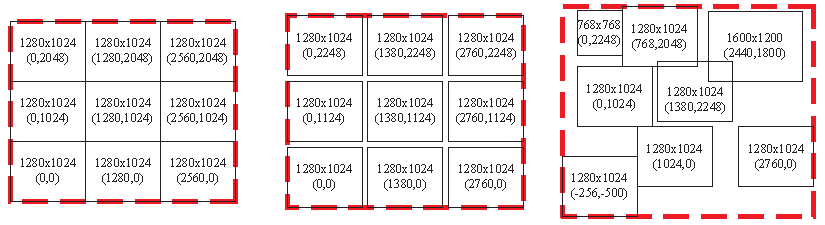
\includegraphics{images/ExampleTileConfig}
  \caption[Defining a tile display.]{Defining a tile display with viewports
    in a logical global display.  Three possible tile arrangements are
    shown.  The bounds of each tile is drawn with the viewport given
    inside.  The viewable area is shown with a dashed line.}
  \label{fig:BasicUsage:tile_layout}
\end{figure}

Figure~\ref{fig:BasicUsage:tile_layout} shows some possible tile
arrangements.  Mullions or overlaps of the tiles in the physical display
can be represented by the spacing or overlap of the viewports in the
logical display.  \IceT does not require the tile layout to have any
regularity.  Chaotic layouts like that shown in the right image of
Figure~\ref{fig:BasicUsage:tile_layout} are legal, although probably not
very useful.  It is allowed, and in fact encouraged, to have processes that
are not directly connected to the tiled display.  These
\index{non-display~process}\keyterm{non-display} processes still contribute
to the image compositing work and will reduce the overall time to render an
image.

The display is defined using the \CFunc{icetResetTiles} and
\CFunc{icetAddTile} functions.  Any previous tile definition is first
cleared out using \CFunc{icetResetTiles} and new tiles are added, one at a
time, using \CFunc{icetAddTile}.

\begin{Table}{3}
  \textC{void }\CFunc{icetResetTiles}\textC{(}&\textC{void}&\textC{)}
\end{Table}

\begin{Table}{3}
  \textC{int }\CFunc{icetAddTile}\textC{(}&\textC{GLint}&\CArg{x}\textC{,} \\
    &\textC{GLint}&\CArg{y}\textC{,} \\
    &\textC{GLsizei}&\CArg{width}\textC{,} \\
    &\textC{GLsizei}&\CArg{height}\textC{,} \\
    &\textC{int}&\CArg{display\_rank}\quad\textC{);}
\end{Table}

Each tile is specified using screen coordinates in the logical global
display: the position of the lower left corner and the width and height of
the tile.  Each tile also has a \index{display~process}\keyterm{display
  process} associated with it.  After an image is completely rendered and
composited, the screen section belonging to this tile will be placed in the
process at the given rank.

The following code demonstrates a common example for establishing the tile
layout: a grid of projectors.  The arrangement of projectors in this
example assume that the projectors are connected to processes in the order
of left to right and then top to bottom, which is common.  Note, however,
that \IceT defines its logical global display with $y$ values from the
bottom up like OpenGL does.

\begin{code}
  icetResetTiles();
  for (row = 0; row < num_tile_rows; row++) {
      for (column = 0; column < num_tile_columns; column++) {
          icetAddTile(column*TILE_WIDTH, (num_tile_rows-row-1)*TILE_HEIGHT,
                      TILE_WIDTH, TILE_HEIGHT,
                      row*num_tile_columns + column);
      }
  }
\end{code}

\index{mullion}\keyterm{Mullions} are added by simply spacing the tiles
apart from each other in the logical global display.  Because they are
defined in the logical global display, physical dimensions of the mullions
must first be converted to pixels using the dot pitch of the displays.  The
following code adds mullions between all of the tiles.

\begin{code}
  icetResetTiles();
  for (row = 0; row < num_tile_rows; row++) {
      for (column = 0; column < num_tile_columns; column++) {
          icetAddTile(column*(TILE_WIDTH + x_mullion),
                      (num_tile_rows-row-1)*(TILE_HEIGHT + y_mullion),
                      TILE_WIDTH, TILE_HEIGHT,
                      row*num_tile_columns + column);
      }
  }
\end{code}

An equally common use for \IceT is to render images in parallel to a single
display.  In this \index{single-tile~rendering}\keyterm{single-tile
  rendering} mode, we simply create a single tile whose image will be
placed in the GUI of some application.  This is done by either using the
OpenGL context of the GUI as part of the \IceT rendering process or by
grabbing the image of the single tile and copying into the GUI.  The
example code below sets up \IceT to create a single image that is
accessible on the root process.

\begin{code}
  icetResetTiles();
  icetAddTile(0, 0, SCREEN_WIDTH, SCREEN_HEIGHT, 0);
\end{code}

\IceT indexes the tiles in the order that they are defined with
\CFunc{icetAddTile}.  You can get the current definition of the tile
display from a number of state variables, which can be retrieved as always
with \CFunc{icetGet}.  \CEnum{ICET\_NUM\_TILES} stores the number of tiles
that are defined (the number of times \CFunc{icetAddTile} was called).
\CEnum{ICET\_TILE\_VIEWPORTS} stores an array with all of the dimensions of
each tile.  For each tile, \CEnum{ICET\_TILE\_VIEWPORTS} contains the four
values $\langle x, y, width, height \rangle$, stored consecutively,
corresponding to the values passed to \CFunc{icetAddTile}.
\CEnum{ICET\_DISPLAY\_NODES} stores an array giving the rank of the
\index{display~process}display process displaying that tile.  Each process
can also query the \CEnum{ICET\_TILE\_DISPLAYED} variable to see which tile
is displayed locally.  \CEnum{ICET\_TILE\_DISPLAYED} is set to $-1$ on
every process that does not display a tile.

You can get information about the display geometry as a whole through
\CEnum{ICET\_GLOBAL\_VIEWPORT}.  This variable stores the four-tuple
$\langle x, y, width, height \rangle$.  $x$ and $y$ are placed at the
leftmost and lowest position of all the tiles, and $width$ and $height$ are
just big enough for the viewport to cover all tiles.

Calling \CFunc{icetAddTile} will not create a display context for the tile.
That responsibility is left to the calling application.  \IceT will use
whatever \index{context!OpenGL}OpenGL context is current.  When using \IceT
in \index{single-tile~rendering}single-tile rendering mode, the OpenGL
context should simply be set to the image size.  When driving a physical
tile display, each display process must create a window that covers the
entire display.  It is also a good idea to disable the mouse cursor in
these windows.

Note that the size of the tiles do not have to match each other.  Also, the
size of the OpenGL viewport does not have to match the size of any of the
tiles.  There is, however, a constraint that the OpenGL viewport on all
processes must be at least as large as the largest tile in each dimension.
To help you maintain that constraint, \IceT stores the largest tile
dimensions in the \CEnum{ICET\_TILE\_MAX\_WIDTH} and
\CEnum{ICET\_TILE\_MAX\_HEIGHT} state variables.  The overall maximum tile
size is provided in \CEnum{ICET\_TILE\_MAX\_PIXELS} so that you can
allocate buffers big enough for any tile image.

Although counterintuitive, it is often more efficient to create OpenGL
viewports that are larger than any tile.  This situation may be necessary
when using \index{image~inflation}image inflation (see
Chapter~\ref{sec:Customizing_Compositing:Image_Inflation}).  Even when not
using image inflation, larger rendering viewports can save a significant
amount of rendering time.  \IceT can use the larger OpenGL image buffer to
potentially render in one shot an object that is larger than any of the
tiles.

\index{display~definition|)}
\index{tile~definition|)}


\section{Strategies}
\label{sec:Basic_Usage:Strategies}

\index{strategy|(}

\IceT contains several algorithms for performing image compositing.  The
overall algorithm used to render and composite an image is called a
strategy, named after the ``Gang of Four'' strategy pattern.\footnote{Erich
  Gamma, Richard Helm, Ralph Johnson, and John Vlissides.  \emph{Design
    Patterns}.  Addison-Wesley, 1994.  ISBN 0-201-63361-2.}  The strategy
is set using the \CFunc{icetStrategy} function.

\begin{Table}{3}
  \textC{void }\CFunc{icetStrategy}\textC{(}&\CType{IceTStrategy}&\CArg{strategy}\quad\textC{);}
\end{Table}

\IceT defines the following strategies that can be passed to
\CFunc{icetStrategy}.  These strategies are discussed in more detail in
Chapter~\ref{chap:Strategies}.

\begin{description}
\item[\CEnum{ICET\_STRATEGY\_REDUCE}]\index{strategy!reduce}
  A two phase algorithm.  In the first phase, tile images are redistributed
  such that each process has one image for one tile.  In the second phase,
  a `traditional' single tile composition is performed for each tile.
  Since each process contains an image for only one tile, all these
  compositions may happen simultaneously.  This is a well rounded strategy
  that seems to perform well in a wide variety of applications.
\item[\CEnum{ICET\_STRATEGY\_SPLIT}]\index{strategy!split} Each tile is
  split up, and each process is assigned a piece of a tile in such a way
  that each process receives and handles about the same amount of data.
  This strategy is often very efficient, but due to the large amount of
  messages passed, it has not proven to be very scalable or robust.
\item[\CEnum{ICET\_STRATEGY\_VTREE}]\index{strategy!virtual~trees} An
  extension to the binary tree algorithm for image composition.  Sets up a
  ``virtual'' composition tree for each tile image.  Processes that belong
  to multiple trees (because they render to more than one tile) are allowed
  to float between trees.  This strategy is not quite as well load balanced
  as \CEnum{ICET\_STRATEGY\_REDUCE} or \CEnum{ICET\_STRATEGY\_SPLIT}, but
  has very well behaved network communication.
\item[\CEnum{ICET\_STRATEGY\_SERIAL}]\index{strategy!serial} Basically
  applies a ``traditional'' single tile composition (such as binary swap)
  to each tile in the order they were defined.  Because each process must
  take part in the composition of each tile regardless of whether they draw
  into it, this strategy is usually very inefficient when compositing for
  more than tile.  It is provided mostly for comparative purposes.
\item[\CEnum{ICET\_STRATEGY\_DIRECT}]\index{strategy!direct} As each
  process renders an image for a tile, that image is sent directly to the
  process that will display that tile.  This usually results in a few
  processes receiving and processing the majority of the data, and is
  therefore usually an inefficient strategy.
\end{description}


\index{strategy|)}

\section{Drawing Callback}
\label{sec:Basic_Usage::Drawing_Callback}

\index{drawing~callback|(}

Most compositing engines will simply take a group of images and combine them
together.  This approach, however, is unreasonable when compositing the
high resolution images on a large tiled display.  It is problematic for an
application to create images larger than any color buffer the rendering
hardware can create, and holding many of these large images can lead to a
large memory profile.

Instead, the \IceT algorithms deal with pieces of the overall image.  The
image pieces are created on demand.  As such, \IceT may require the same
geometry to be rendered multiple times in a single frame.  \IceT provides
the application with the most flexible way to define the rendering process:
with a \keyterm{drawing callback}.

A drawing callback is simply a function that your application provides
\IceT.  When \IceT needs an image, it will establish the appropriate OpenGL
transformation matrices for the section of the overall display it needs.
The application's drawing callback will issue the appropriate OpenGL
commands to draw the geometry.  The drawing callback leaves its image in
the OpenGL buffers upon exiting.

The drawing callback is set with the \CFunc{icetDrawFunc}.

\textC{typedef void (*}\CType{IceTCallback}\textC{)(void);}

\begin{Table}{3}
  \textC{void }\CFunc{icetDrawFunc}\textC{(}&\CType{IceTCallback}&\CArg{func}\quad\textC{);}
\end{Table}

\IceT can nominally call the drawing callback for every tile in the
display.  However, in almost any real application each process has data
that demonstrates some spatial locality that causes it to be projected on a
relatively small section of the display.  To give \IceT the information it
needs to prevent unnecessary renders, the application needs to provide the
bounds of the local geometry.  This is done using either the
\CFunc{icetBoundingVertices} or the \CFunc{icetBoundingBox} function.

\begin{Table}{3}
  \textC{void }\CFunc{icetBoundingVertices}\textC{(}&\textC{GLint}&\CArg{size}\textC{,} \\
    &\textC{GLenum}&\CArg{type}\textC{,} \\
    &\textC{GLsizei}&\CArg{stride}\textC{,} \\
    &\textC{GLsizei}&\CArg{count}\textC{,} \\
    &\textC{const GLvoid *}&\CArg{pointer}\quad\textC{);}
\end{Table}

\begin{Table}{3}
  \textC{void }\icetBoundingBoxd\textC{(}&\textC{GLdouble}&\CArg{x\_min}\textC{,} \\
    &\textC{GLdouble}&\CArg{x\_max}\textC{,} \\
    &\textC{GLdouble}&\CArg{y\_min}\textC{,} \\
    &\textC{GLdouble}&\CArg{y\_max}\textC{,} \\
    &\textC{GLdouble}&\CArg{z\_min}\textC{,} \\
    &\textC{GLdouble}&\CArg{z\_max}\quad\textC{);}
\end{Table}

\begin{Table}{3}
  \textC{void }\icetBoundingBoxf\textC{(}&\textC{GLfloat}&\CArg{x\_min}\textC{,} \\
    &\textC{GLfloat}&\CArg{x\_max}\textC{,} \\
    &\textC{GLfloat}&\CArg{y\_min}\textC{,} \\
    &\textC{GLfloat}&\CArg{y\_max}\textC{,} \\
    &\textC{GLfloat}&\CArg{z\_min}\textC{,} \\
    &\textC{GLfloat}&\CArg{z\_max}\quad\textC{);}
\end{Table}

With the \CFunc{icetBoundingVertices} function, you specify a set of
vertices whose convex hull completely contains the geometry.  The
\CFunc{icetBoundingBox} function is a convenience function that defines the
container as an axis aligned bounding box.

The drawing callback should \emph{not} modify the
\CEnum{GL\_PROJECTION\_MATRIX} as this would cause \IceT to place image
data in the wrong location in the tiled display and improperly cull
geometry.  It is acceptable to add transformations to
\CEnum{GL\_MODELVIEW\_MATRIX}, but the bounding vertices given with
\CFunc{icetBoundingVertices} or \CFunc{icetBoundingBox} are assumed to
already be transformed by any such changes to the modelview matrix.  Also,
\CEnum{GL\_MODELVIEW\_MATRIX} must be restored before the draw function
returns.  Therefore, any changes to \CEnum{GL\_MODELVIEW\_MATRIX} are to be
done with care and should be surrounded by a pair of glPushMatrix and
glPopMatrix functions.

It is also important that the drawing callback \emph{not} attempt the
change the clear color.  In some compositing modes, \IceT needs to read,
modify, and change the background color.  These operations will be lost if
the drawing callback changes the background color, and severe color
blending artifacts may result.

\IceT may call the drawing callback several times to create a single tiled
image or not at all if the current bounds lie outside the current
view frustum.  This can have a subtle but important impact on the behavior of
the drawing callback.  For example, counting frames by incrementing a frame
counter in the drawing callback is obviously wrong (although you could
count how many times a render occurs).  The drawing callback should also
leave \OpenGL in a state such that it will be correct for a subsequent run
of the drawing callback.  Any matrices or attributes pushed in the drawing
callback should be popped before the drawing callback returns, and any
state that is assumed to be true on entrance to the drawing callback should
also be true on return.

\index{drawing~callback|)}


\section{Rendering}
\label{sec:Basic_Usage:Rendering}

Once you have set up the \IceT state as described in the previous sections
of this chapter, you are ready to perform parallel rendering.  Parallel
rendering is performed by calling \CFunc{icetDrawFrame}.

\begin{Table}{3}
  \textC{void }\CFunc{icetDrawFrame}\textC{(void);}
\end{Table}

\CFunc{icetDrawFrame} is called in basically the same way as the
\index{drawing~callback}drawing callback would be called directly.  First,
establish the OpenGL state.  Setting up the \CEnum{GL\_PROJECTION\_MATRIX}
before calling \CFunc{icetDrawFrame} is essential.  It is also advisable to
set up whatever transformations in the \CEnum{GL\_MODELVIEW\_MATRIX} that
you can before calling \CFunc{icetDrawFrame}.  \IceT will use and modify
these two matrices to render regions of the tiled display.  The drawing
callback should behave as if neither of the matrices were modified.

By the time \CFunc{icetDrawFrame} completes, an image will have been
completely rendered and composited.  If \CEnum{ICET\_DISPLAY} is enabled,
then the fully composited image is written back to the \OpenGL framebuffer
for display.  It is the application's responsibility to synchronize the
processes and swap front and back buffers.  The image remaining in the
frame buffer is undefined if \CEnum{ICET\_DISPLAY} is disabled or the
process is not displaying a tile.

If the \OpenGL background color is set to something other than black,
\CEnum{ICET\_DISPLAY\_COLORED\_BACKGROUND} should also be enabled.
Displaying with \CEnum{ICET\_DISPLAY\_COLORED\_BACKGROUND} disabled may be
slightly faster (depending on graphics hardware) but can result in black
rectangles in the background.

If \CEnum{ICET\_DISPLAY\_INFLATE} is enabled and the size of the renderable
window (determined by the current \OpenGL viewport) is greater than that of
the tile being displayed, then the image will first be ``inflated'' to the
size of the actual display.  If \CEnum{ICET\_DISPLAY\_INFLATE} is disabled,
the image is drawn at its original resolution at the lower left corner of
the display.  More details on image inflation are given in
Chapter~\ref{sec:Customizing_Compositing:Image_Inflation}.

Regardless of whether it writes the fully composited image back to the
display, \IceT stores the resulting image buffers.  These image buffers can
be retrieved with the \icetGetColorBuffer and \icetGetDepthBuffer
functions.

\begin{Table}{4}
  \textC{GLubyte}&\textC{*}\icetGetColorBuffer&\textC{(}&\textC{void}\quad\textC{)}; \\
  \textC{GLuint}&\textC{*}\icetGetDepthBuffer&\textC{(}&\textC{void}\quad\textC{)}; \\
\end{Table}

Of course, color buffers are only available on
\index{display~process}display processes.  Also be aware that a color or
depth buffer may not have been computed with the last call to
\CFunc{icetDrawFrame}.  \IceT avoids the computation and network transfers
for any unnecessary buffers unless specifically requested otherwise with
the flags given to the \CFunc{icetInputOutputBuffers} function.

\begin{Table}{3}
  \textC{void }\CFunc{icetInputOutputBuffers}\textC{(}&\textC{GLenum}&\CArg{inputs}\textC{,} \\
    &\textC{GLenum}&\CArg{outputs}\quad\textC{);}
\end{Table}

\CFunc{icetInputOutputBuffers} allows you to specify which OpenGL buffers
to composite (the \CArg{input} buffers) and which to deliver to the
\index{display~process}display processes (the \CArg{output} buffers).  The
color and depth buffers are specified with the
\CEnum{ICET\_COLOR\_BUFFER\_BIT} and \CEnum{ICET\_DEPTH\_BUFFER\_BIT},
respectively.  By default, \IceT reads in both the color and depth buffers,
performs compositing using \index{Z~comparison}\keyterm{Z comparison}, and
delivers just the color buffer to the display nodes.  If you need the depth
buffer as well, specify depth as one of the outputs.  If you do not need
the color buffer, you can remove the color buffer as one of the input
buffers.  If the depth buffer is not specified as one of the inputs, then
the compositing mode is automatically switched to
\index{alpha~blending}\keyterm{alpha blending}.  However, alpha blending
requires additional information from the application, which is discussed
in Chapter~\ref{sec:Customizing_Compositing:Volume_Rendering}.

In any case, you can query whether a color or depth buffer is available
with \CEnum{ICET\_COLOR\_BUFFER\_VALID} or
\CEnum{ICET\_DEPTH\_BUFFER\_VALID}, respectively.  It is an error to read
an invalid buffer.

The memory returned by \icetGetColorBuffer and \icetGetDepthBuffer need
not, and should not, be freed.  It will be reclaimed in the next call to
\CFunc{icetDrawFrame}.  Expect the data returned to be obliterated on the
next call to \CFunc{icetDrawFrame}.
